\documentclass[varwidth=\maxdimen]{standalone}
\usepackage{tikz}
\usetikzlibrary{fit}
\usepackage[nomessages]{fp}

\tikzset{every label/.style={font=\footnotesize,inner sep=1.5pt}}

\newcommand{\pc}[4][]{\node[circle, fill, label={below:#4},#1] at (#2) (#3) {}}
\newcommand{\pcghost}[4][]{\node[circle, fill=gray, label={below:#4},#1] at (#2) (#3) {}}
\newcommand{\pu}[4][]{\node[rectangle, fill=blue, label={above:#4},#1] at (#2) (#3) {}}
\newcommand{\pughost}[4][]{\node[rectangle, fill=gray, label={above:#4},#1] at (#2) (#3) {}}
\newcommand{\pv}[4][]{\node[rectangle, fill=red, label={below:#4},#1] at (#2) (#3) {}}
\newcommand{\nx}{8} %number of cells in x direction
\newcommand{\ny}{8} %number of cells in y direction
\newcommand{\nghost}{3} %number of ghost cells in x direction
\newcommand{\xmin}{0}  %grid start
\newcommand{\xmax}{12} %grid end
\newcommand{\ymin}{0}  %grid start
\newcommand{\ymax}{12} %grid end

\begin{document}
	\begin{figure}[h]
		\centering
		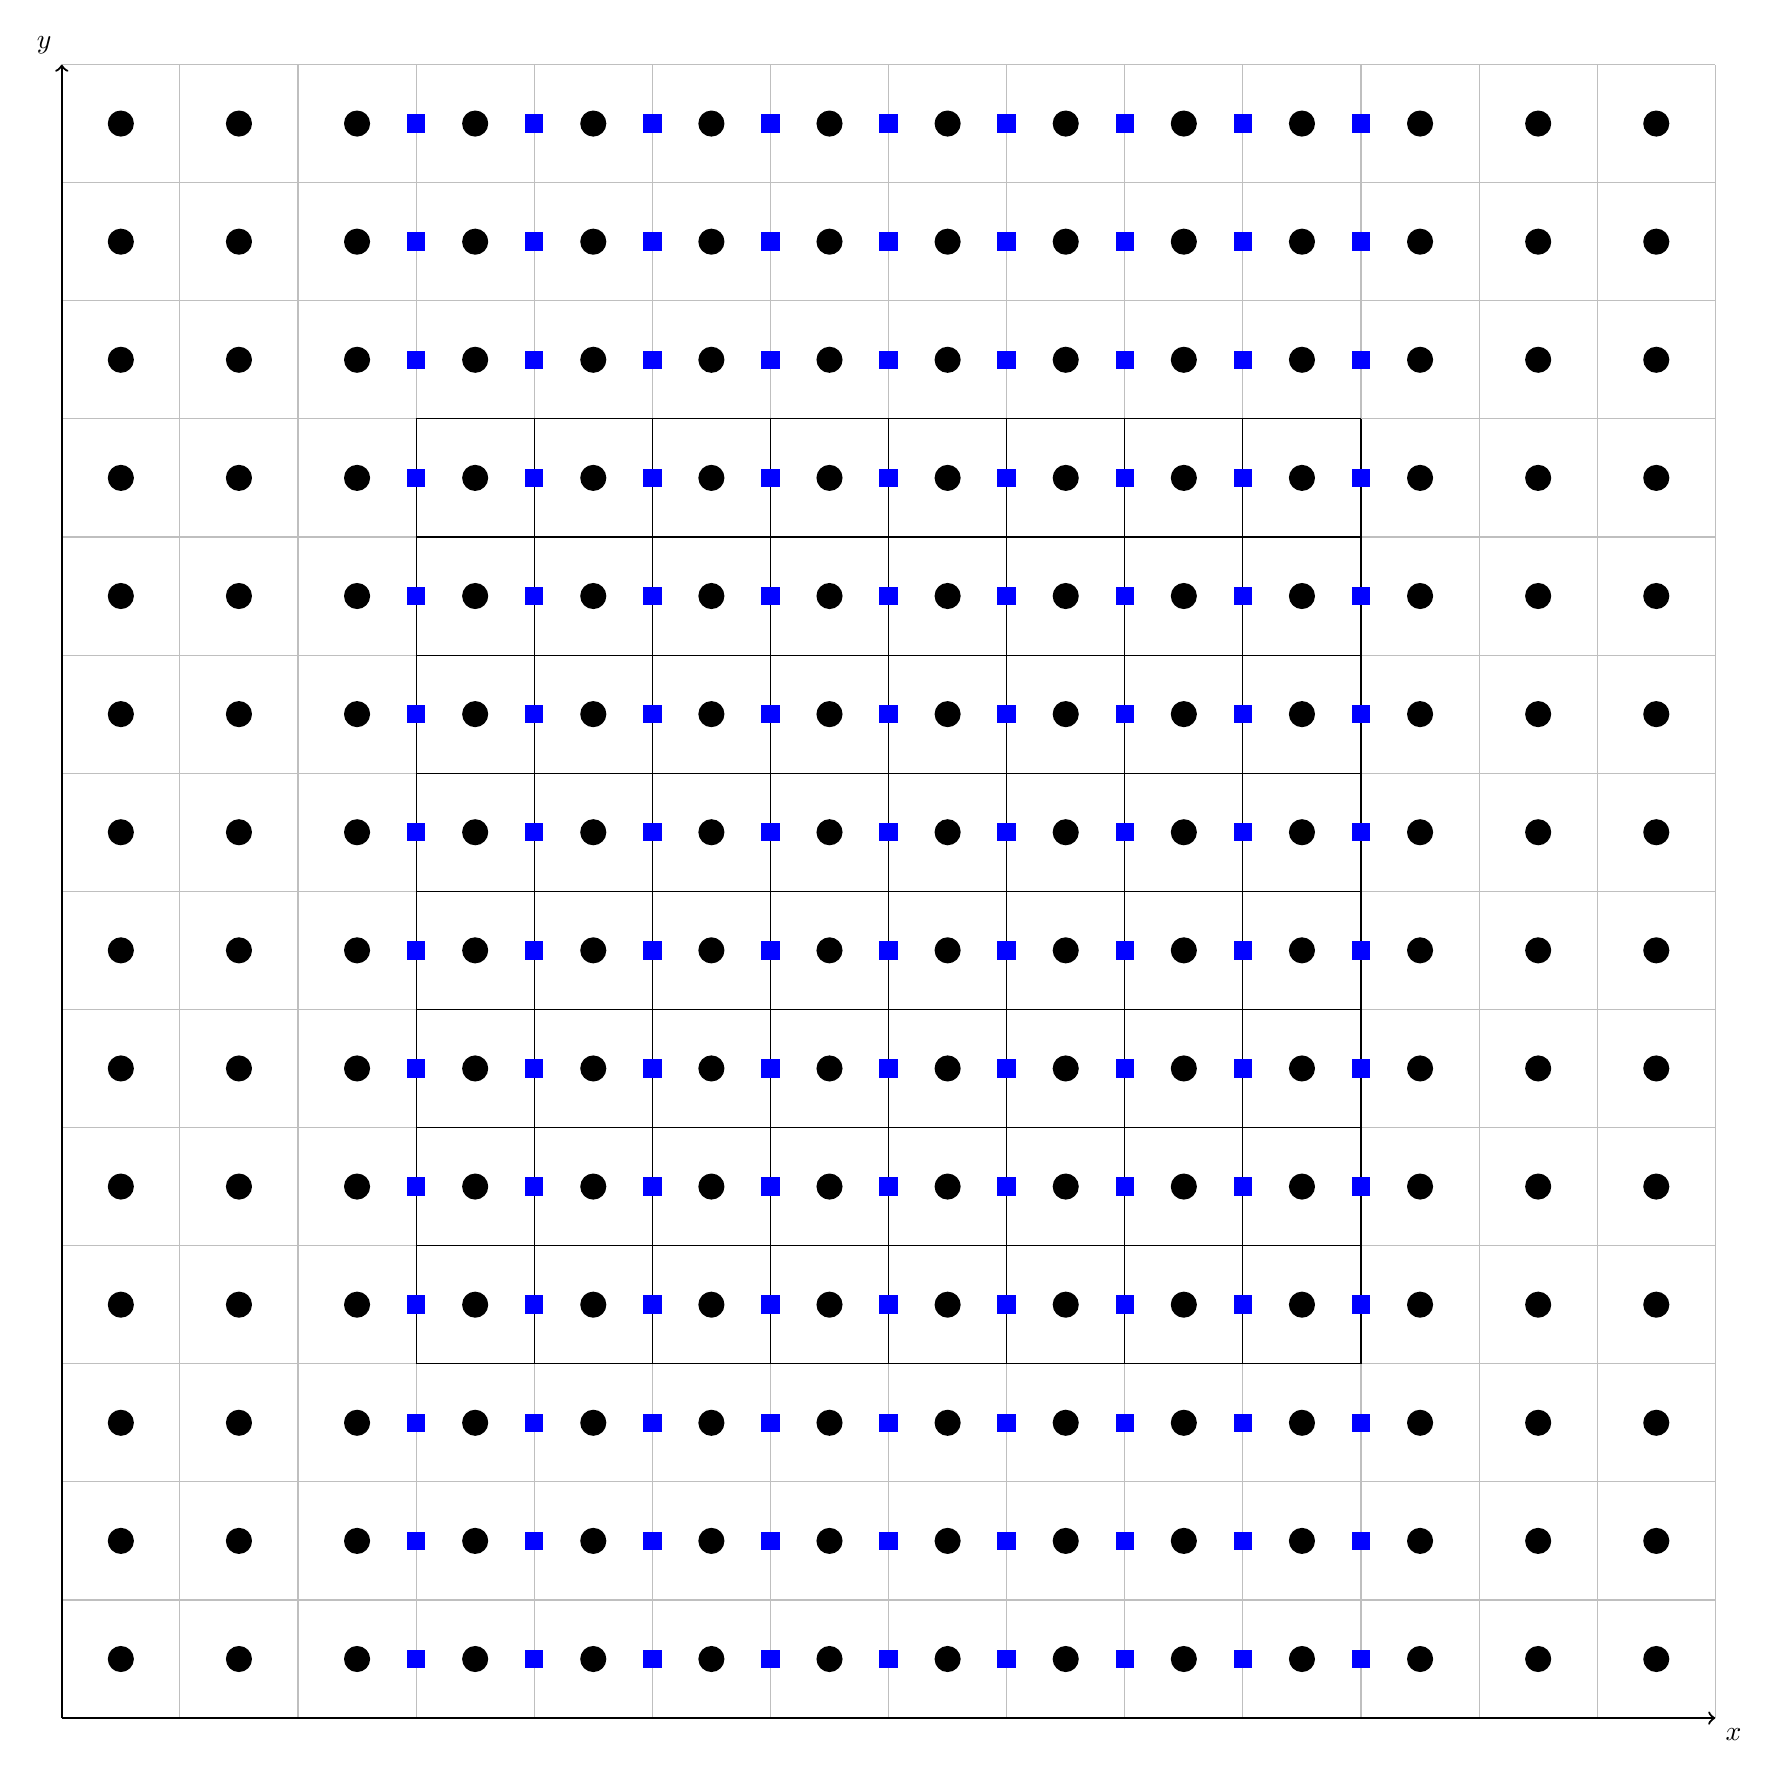
\begin{tikzpicture}
			% Grid lines
			%%%%%%%%%%%%%%%%%%%%%%%%%%%%%%%%%%%%%%%%%%%%%%%%%%%%%%%%%%%%%%%
			\FPeval{\dx}{clip((\xmax-\xmin)/\nx)}
			\FPeval{\dy}{clip((\ymax-\ymin)/\ny)}
			\FPeval{\istart}{clip(-nghost)}
			\FPeval{\iend}{clip(\nx+\nghost)}
			\foreach \i in {\istart,...,\iend}{
				\FPeval{\xp}{clip(\xmin+\i*\dx)}					
				\draw[gray!50, thin] (\xp,\ymin -\nghost*\dy)--(\xp,\ymax+\nghost*\dy);
				\draw[gray!50, thin] (\ymin -\nghost*\dy,\xp)--(\ymax+\nghost*\dy,\xp);
			}


			\foreach \i in {0,...,\nx}{
				\FPeval{\xp}{clip(\xmin+\i*\dx)}					
				\draw[black!100, thin] (\xp,\ymin)--(\xp,\ymax);
				\draw[black!100, thin] (\ymin,\xp)--(\ymax,\xp);
			}

			% Interior grid centers
			\FPeval{\istart}{clip(-\nghost+1)}
			\FPeval{\iend}{clip(\nx+\nghost)}
			\FPeval{\jstart}{clip(-\nghost+1)}
			\FPeval{\jend}{clip(\ny+\nghost)} 
			\foreach \i in {\istart,...,\iend}{
				\FPeval{\xp}{clip(\xmin+(\i-0.5)*\dx)}
				\foreach \j in {\jstart,...,\jend}{
					\FPeval{\yp}{clip(\ymin+(\j-0.5)*\dy)}
					\pc{\xp,\yp}{5}{};
				}
			}

			% Interior grid edge midpoints
			\FPeval{\jstart}{clip(-\nghost+1)}
			\FPeval{\jend}{clip(\ny+\nghost)} 
			\foreach \i in {0,...,\nx}{
				\FPeval{\xc}{clip(\xmin+\i*\dx)}
				\foreach \j in {\jstart,...,\jend}{
					\FPeval{\yc}{clip(\ymin+(\j-0.5)*\dy)}
					\pu{\xc,\yc}{5}{};
				}
			}


% X-axis
\draw[->, thick] (\xmin-\nghost*\dx,\ymin-\nghost*\dy) -- (\xmax+\nghost*\dx,\ymin-\nghost*\dy) node[below right] {$x$};
% Y-axis
\draw[->, thick] (\xmin-\nghost*\dx,\ymin-\nghost*\dy) -- (\xmin-\nghost*\dx,\ymax+\nghost*\dy) node[above left] {$y$};

		\end{tikzpicture}
	\end{figure}
\end{document}
